\section{Exploration on Human Occupancy Behaviour}
\label{sec:exploration}

Up to this point, this paper has been concerned with Bayesian methods for correctly estimating count data. The application to these methods is used to correctly estimate human occupancy behaviour in a certain place at a particular time given that available sensors in the robot are unreliable. In this part, we used the resulting predictions to drive exploration for human activities. In particular, the aim is to drive the robot to go where there are the most people performing activities, i.e. where the aggregate level of human occupancy is highest. 

\subsection*{Exploration Models}

The problem to create a plan of a series of visits to specific areas which will give the highest number of human occupancy can be seen as an exploration-exploitation problem. This problem is well known in the reinforcement learning community, and it is known as the problem of optimising the exploration-exploitation trade-off. Exploration-exploitation problems arise when an agent, in this scenario the mobile robot acts as the agent, does not fully understand the process it is trying to control. In any time, the robot is given two options. It can either spend its time and resources to better understand the process (explore) for a
better action later on, but sacrificing its short-term reward, or spend its time and resources to exploit what the robot already understands to gain reward and risk permanently following it policy that might be suboptimal. In each time the robot has a choice between many actions, each of which both explores and exploits a certain place, but to varying degrees. As its goal is to maximise the reward gathered–as in getting as much data on human activities (by seeing as many humans) as possible–given its limited operational life, it is preferable to have a policy that is as near optimal as possible.

While exploration-exploitation problems in reinforcement learning are typically intractable, there are well known approximate answers that are very quick to compute \cite{wyatt1998exploration, 1413255, AUDIBERT20091876}. One such answer is to use the upper bound of the probability interval of the arrival rate ($\lambda$) of a Poisson process ($\lambda_{UB}$) to provide areas for the robot to visit. The upper bound of the probability interval of the arrival rate of a Poisson process is calculated as follows

\begin{equation}
	\label{eq:upper_bound_exploration}
	\begin{tabular}{r@{ = }l}
	$\lambda_{UB}(t_i, t_j)$ & $\displaystyle \int_{t_i}^{t_j} CDF^{-1}(\% = 0.95 \mid \alpha_t, \beta_t)~dt$\\ [1ex]
	\end{tabular}
\end{equation}

\noindent with $\lambda_{UB}(t_i, t_j)$ as the upper bound of $\lambda$ within time $t_i$ and $t_j$, $i, j \in \{1, \ldots, \Delta\}$, and $CDF^{-1}$ as the inverse of the cummulative density function of a gamma distribution. Given a series of upper bounds $\lambda^{r}_{UB}(t_i, t_j)$ for each place, places which will be visited between time $t_i$ and $t_j$ is chosen by

\begin{equation}
\label{eq:choosing_place}
\underset{r \in \mathcal R}{\arg\max}~\lambda^{r}_{UB}(t_i, t_j)
\end{equation}
\noindent with $\mathcal R$ as a set of specified places. Figure~\ref{fig:map_vs_ub} depicts a comparison between the MAP hypothesis estimate and the upper bound estimate of a Poisson process.

\begin{figure}[t!]
	\centering
	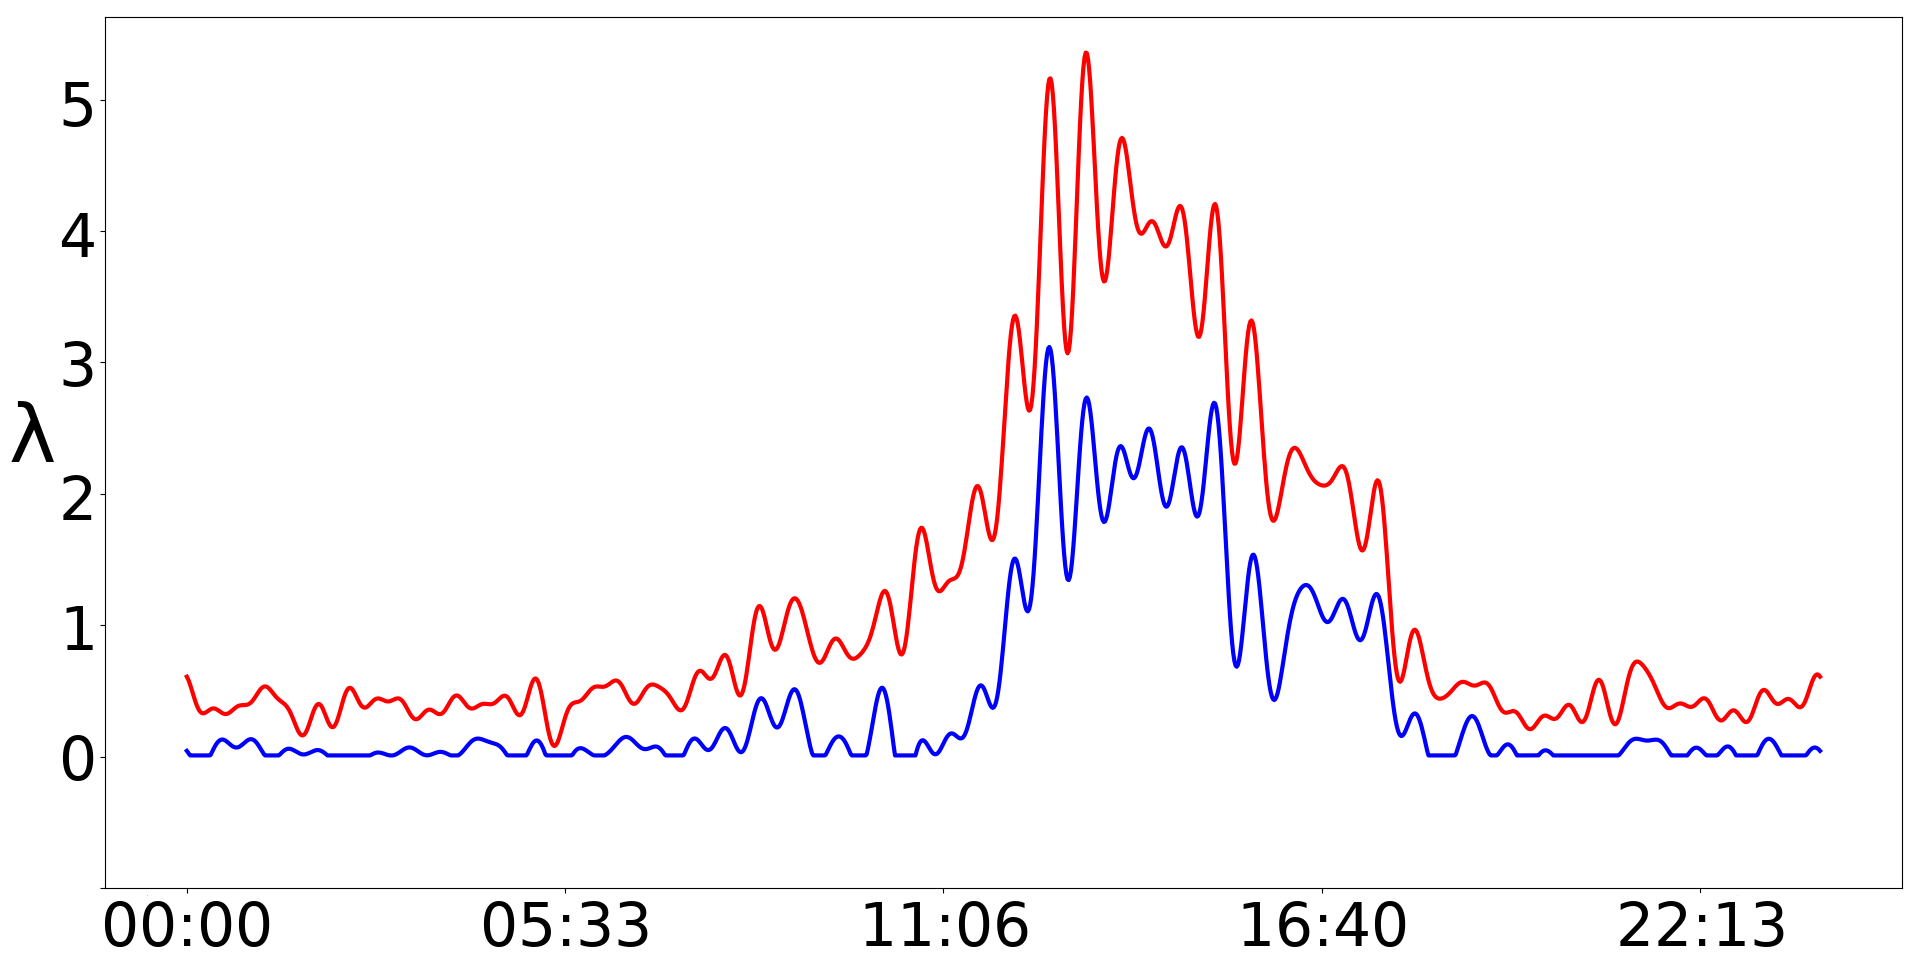
\includegraphics[width=0.5\textwidth]{./figures/map_vs_ub.png}
	\caption{A periodic Poisson process of area 9 (see Figure \ref{fig:map_popp_independent_test}) represented by its MAP hypothesis (blue line) and its upper bound of the probability interval (red line).}
	\label{fig:map_vs_ub}
\end{figure}

These upper bounds $\lambda^{r}_{UB}(t_i, t_j)$ are used in three different exploration models: the spectral-FOPP, the spectral-POPP, and the spectral-POPP-Beta. The spectral-FOPP is an exploration model which follow a periodic Poisson model with Fourier transformation applied to the series of point estimates of the periodic model for getting a smoother model with the periodic set to a daily cycle. This exploration model combines the FOPP model and a spectral analysis, introduced in \cite{jovan_iros16}, together to cope with temporally incomplete data. In this particular case, for the spectral-FOPP exploration model, a series of upper bounds $\lambda_{UB}(t_i, t_j)$ are encoded and extracted via spectral analysis with $l$-AAM technique \cite{jovan_iros16} to produce a smoother series of upper bound estimates $\lambda'_{UB}(t_i, t_j)$. Algorithm 4 depicts the process of choosing the upper bound of $\lambda$ of a Poisson process and applying spectral analysis to it.

\begin{figure}[t!]
	\begin{center}
		\begin{tabular*}{0.5\textwidth}{l @{\extracolsep{\fill}}}
			\hline
			\textbf{Algorithm 4} \textit{Spectral Upper Bound} \\
			\hline
			\textbf{Input:} $(\alpha_1, \beta_1), \ldots, (\alpha_n, \beta_n)$: Poisson process \\
			\textbf{Output:} $\lambda^{ub}_1, \ldots, \lambda^{ub}_n$: spectral upper bound \\
			\textbf{Procedure:}\\
			\hspace{0.3cm} 1. Init. k $\leftarrow$ 1, m $\leftarrow$ $\eta$ \\
			\hspace{0.3cm} 2. Repeat until k $>$ n \\
			\hspace{0.7cm} $\bullet ~ k \leftarrow k + 1$ \\
			\hspace{0.7cm} // Get the upper bound of the confidence interval \\
			\hspace{0.7cm} $\bullet ~ \lambda_k \leftarrow CDF(0.95, \alpha_k, \beta_k)$ \\
			\hspace{0.3cm} // Transform $\lambda_1, \ldots, \lambda_n$ to spectrums with $l$-AAM \\
			\hspace{0.3cm} 3. $\mathcal S$ $\leftarrow$ \textbf{Algorithm1}($\lambda_1, \ldots, \lambda_n$, l) \\
			\hspace{0.3cm} 5. Init. k $\leftarrow$ 1,  $\lambda^{ub}_1, \ldots, \lambda^{ub}_n \leftarrow (0, \ldots, 0)$ \\
			\hspace{0.3cm} 4. Repeat until k $>$ m \\
			\hspace{0.7cm} // Create a cosine signal from $\mathcal S[k]$ \\
			\hspace{0.7cm} $[\mid \omega_k \mid, arg(\omega_k), \omega_k] \leftarrow \mathcal S[\omega_k]$ \\
			\hspace{0.7cm} $\bullet ~ x_1, \ldots, x_n \leftarrow \mid \omega_k \mid * cos(2 \pi * \omega_k + arg(\omega_k))$ \\
			\hspace{0.7cm} // Add current $\lambda^{ub}_1, \ldots, \lambda^{ub}_n$ with the cosine signal \\
			\hspace{0.7cm} $\bullet ~ \lambda^{ub}_1, \ldots, \lambda^{ub}_n \leftarrow \lambda^{ub}_1, \ldots, \lambda^{ub}_n + x_1, \ldots, x_n$ \\
			\hline
		\end{tabular*}	
	\end{center}
\end{figure} 

The spectral-POPP and the spectral-POPP-Beta are the spectral-FOPP exploration model with POPP (or POPP-Beta) estimators applied during the learning / updating process of the model for correcting any systematic error produced by sensors. The switching filter is used for the POPP and POPP-Beta estimators.

\subsection*{Exploration Evaluation}

Lets recall the dataset which had been used in the previous section to assess the accuracy and performance of the POPP model and its extensions. This dataset was, in fact, collected by the exploration models described earlier throughout 69-days of the robot deployment. Due to hardware failures, sensor malfunctions and other external issues related to the mobile robot, only 48 days from the dataset were deemed worth analysis.

Three different exploration models were applied separately during the 69-day of
the deployment. All of these models used $\lambda_{UB}$ for their exploration policies. For the first 27 days of the deployment, the robot followed an exploration policy according to the spectral-FOPP model. This resulted in 18 days worth of data collected. From this 18 days data collected by following the spectral-FOPP exploration model, the last 3 days were used to train the sensor model needed for both the spectral-POPP and the spectral-POPP-Beta models. From day 28 to day 47, the robot followed an exploration policy according to the spectral-POPP model. This resulted in 15 days worth of data collected. Finally, from day 48 onwards, the robot followed an exploration policy according to the spectral-POPP-Beta model. This resulted to 15 days worth of data collected.

A comparison among different exploration policies is made, based on how many observations the robot makes using a particular exploration model. For this comparison, the last 3 days which are part of the 18 days worth of data collected by following the spectral-FOPP exploration model are included in the spectral-POPP and the spectral-POPP-Beta exploration models. This is necessary to avoid the spectral-POPP and the spectral-POPP-Beta exploration models having an advantage over the spectral-FOPP exploration model since the spectral-POPP and the spectral-POPP-Beta need a training period to construct their sensor model. Moreover, due to the absence of information regarding activities happening in other places that the robot did not visit, only a comparison of the total duration of positive observations over the total duration of its visit can be compared and evaluated. As a note, a positive observation is a duration when the robot observes any activity during its visit to a particular area. 

\begin{figure}[t!]
	\centering
	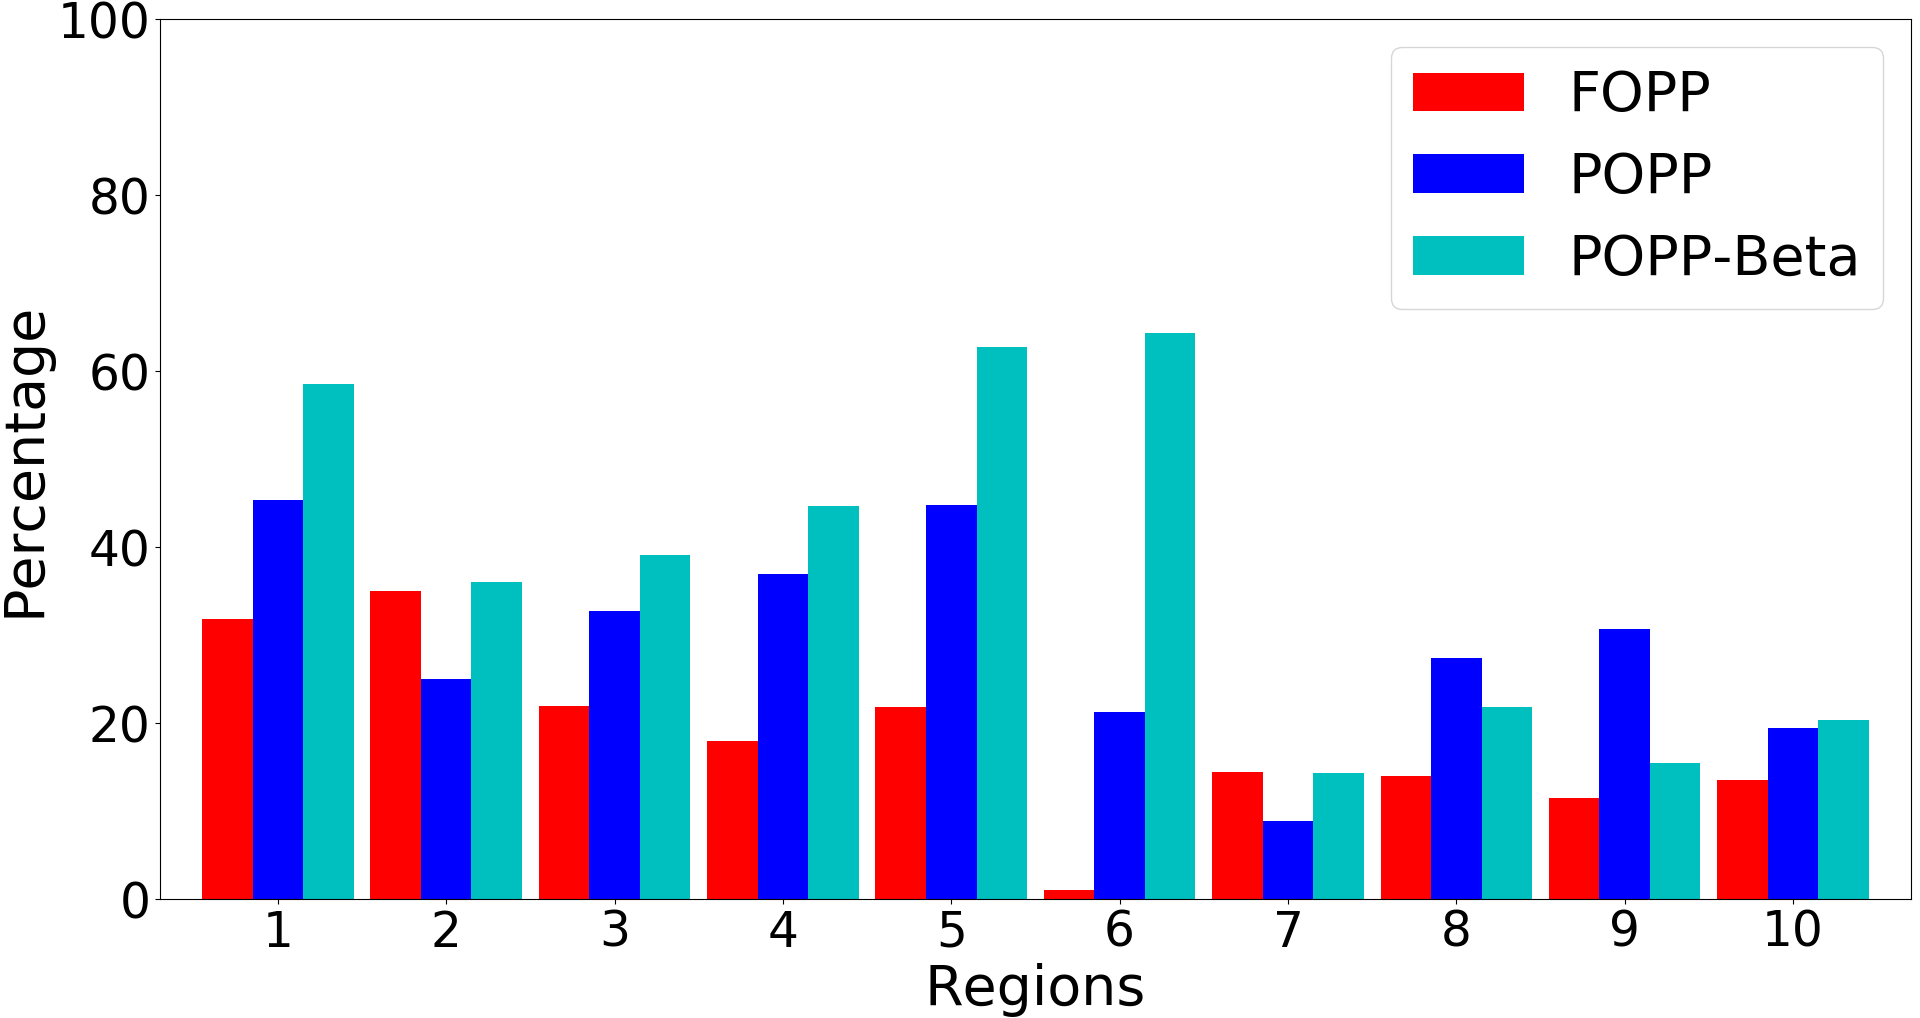
\includegraphics[width=0.5\textwidth]{./figures/exploration_percentage_region.png}
	\caption{The activity exploration percentage across areas of the environment using three different exploration models (spectral-FOPP, spectral-POPP, spectral-POPP-Beta). The percentage shows the portion of time that the robot was observing activities.}
	\label{fig:exploration_percentage_region}
\end{figure}

Figure \ref{fig:exploration_percentage_region} shows the portion of positive observations over the total duration the robot spent in each area of the environment. As can be seen, the exploration policy produced by spectral-POPP-Beta has the highest positive observations in many of the regions followed by the exploration policy according to the spectral-POPP model. Recall that some regions, such as 4, 5, 6, and 7, are not densely populated with humans across time compared to other regions (such as 1, 2, 3, and 10). The spectral-POPP and spectral-POPP-Beta models, however, still managed to improve the percentage of positive observations. This showed that the models correctly predicted that activities would take place in particular locations. One should note that region 6 is the place where there are vending machines. These are often detected as a person by the upper body detector attached to the robot. This might lead the spectral-FOPP model to plan a visit to this particular location when no activity takes place. As can be seen, the spectral-POPP and the spectral-POPP-Beta models were able to correct the miscounts occurring in region 6, and also giving a better estimate to the posterior over the arrival rate $\lambda$ and thus making the exploration-exploitation trade-off using better beliefs.